\documentclass[crop=false, class=book]{standalone}


\usepackage{graphicx}
\usepackage[italian]{varioref}
\usepackage{copyrightbox}
\usepackage{subfig}


\begin{document}

	\chapter{User Interaction}
	ARCore utilizza la tecnologia \textit{ray casting} per permettere all'utente di posizionare un oggetto nella scena corrente in un punto fissato. Quando lo schermo del telefono viene toccato o viene compiuta qualche altra interazione, viene proiettato un raggio nella visuale del mondo della fotocamera che può intersecare un preciso punto o piani geometrici. ARCore permette di ricavare un elenco dei risultati delle intersezioni con la geometria della scena rilevata attraverso gli hitTest. Solitamente il primo risultato è quello più significativo perchè si riferisce all'intersezione più vicina al dispositivo.
	
	\begin{figure}[h]
			\centering
			\subfloat[][]
			{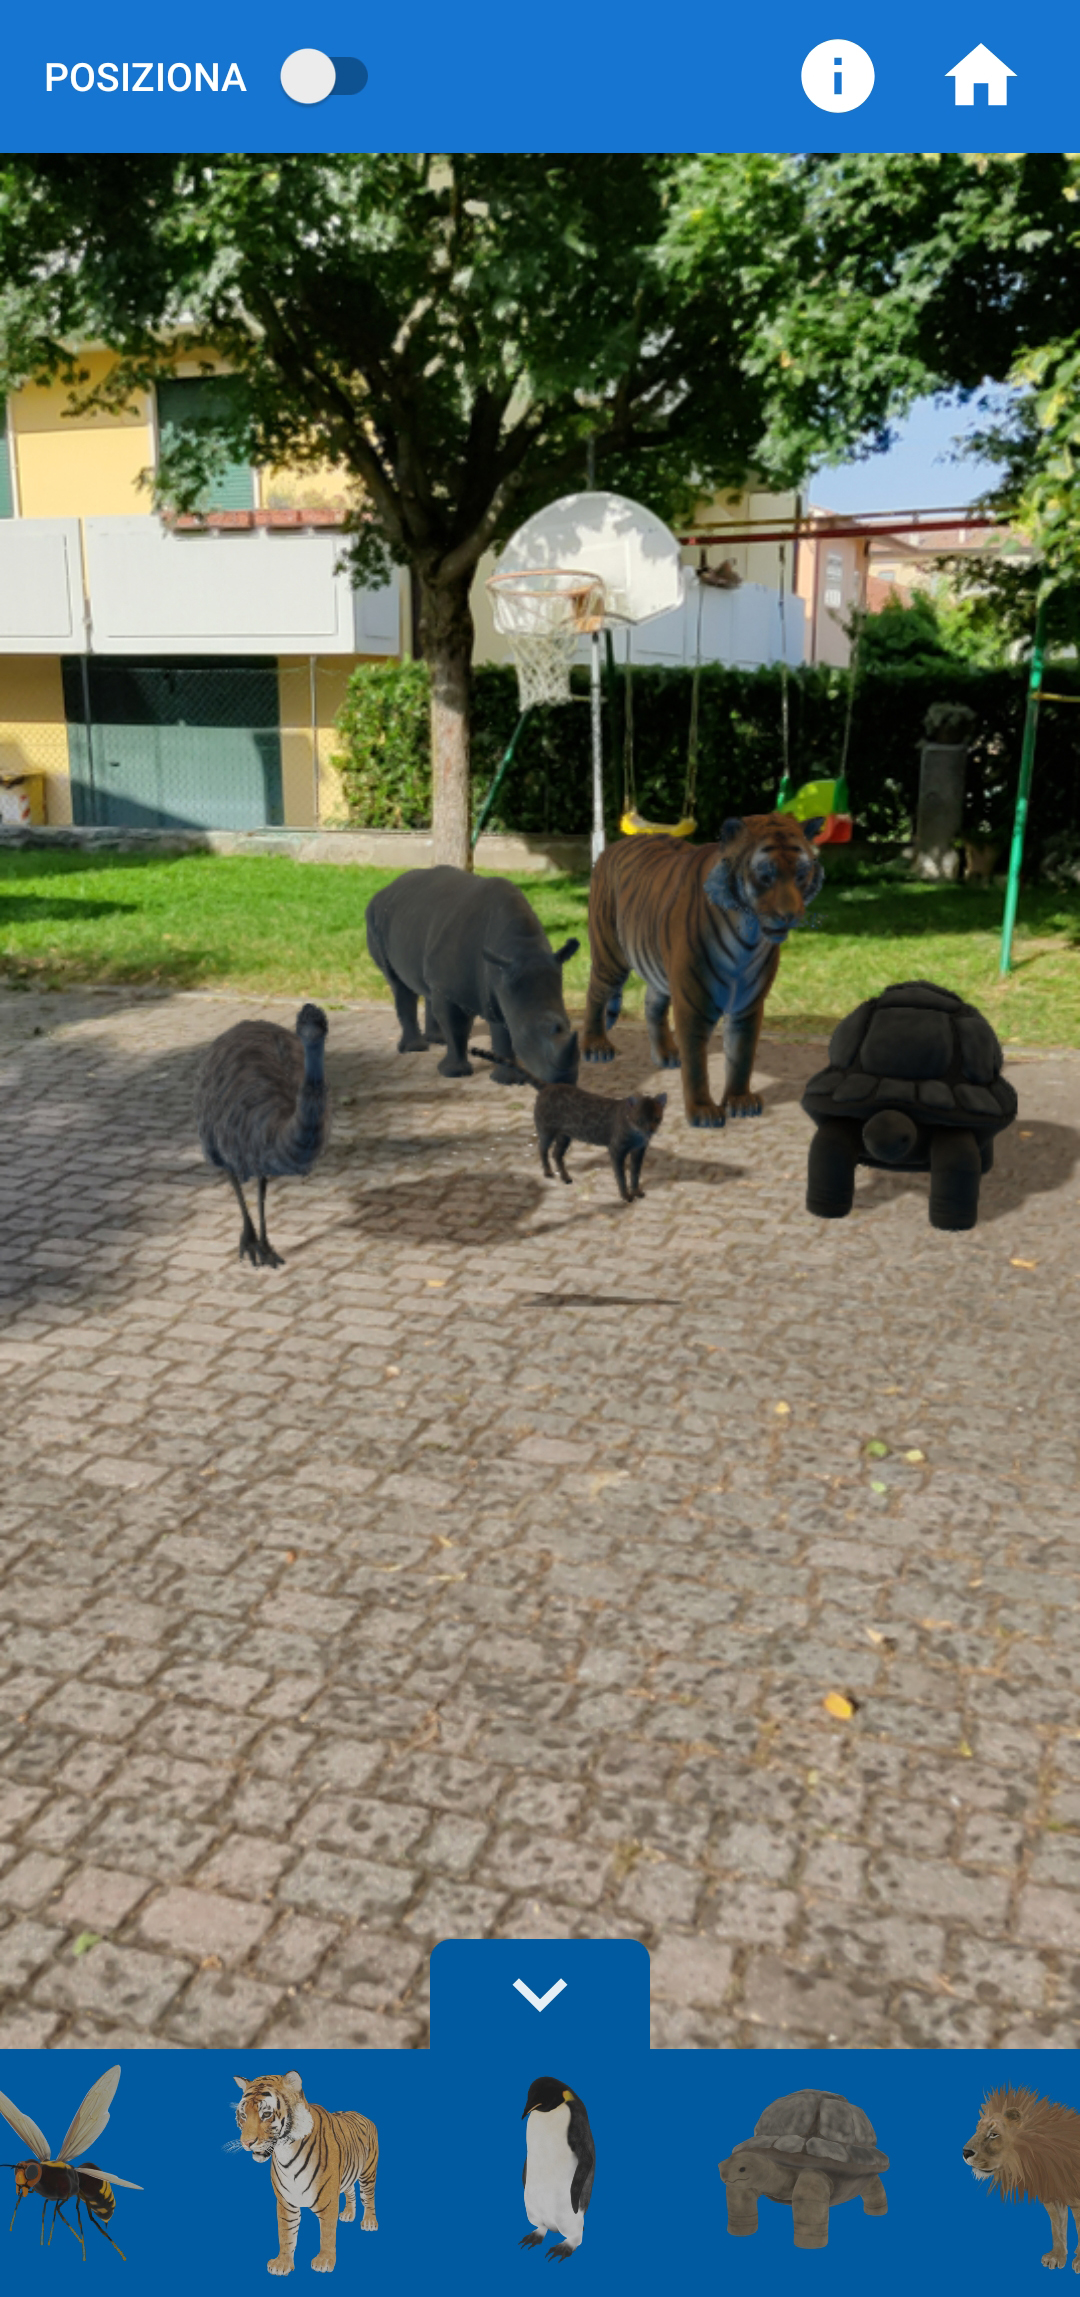
\includegraphics[width=0.3\textwidth]{./resources/images/UserInteraction/Animals1.jpg}}  \qquad
			\subfloat[][]
			{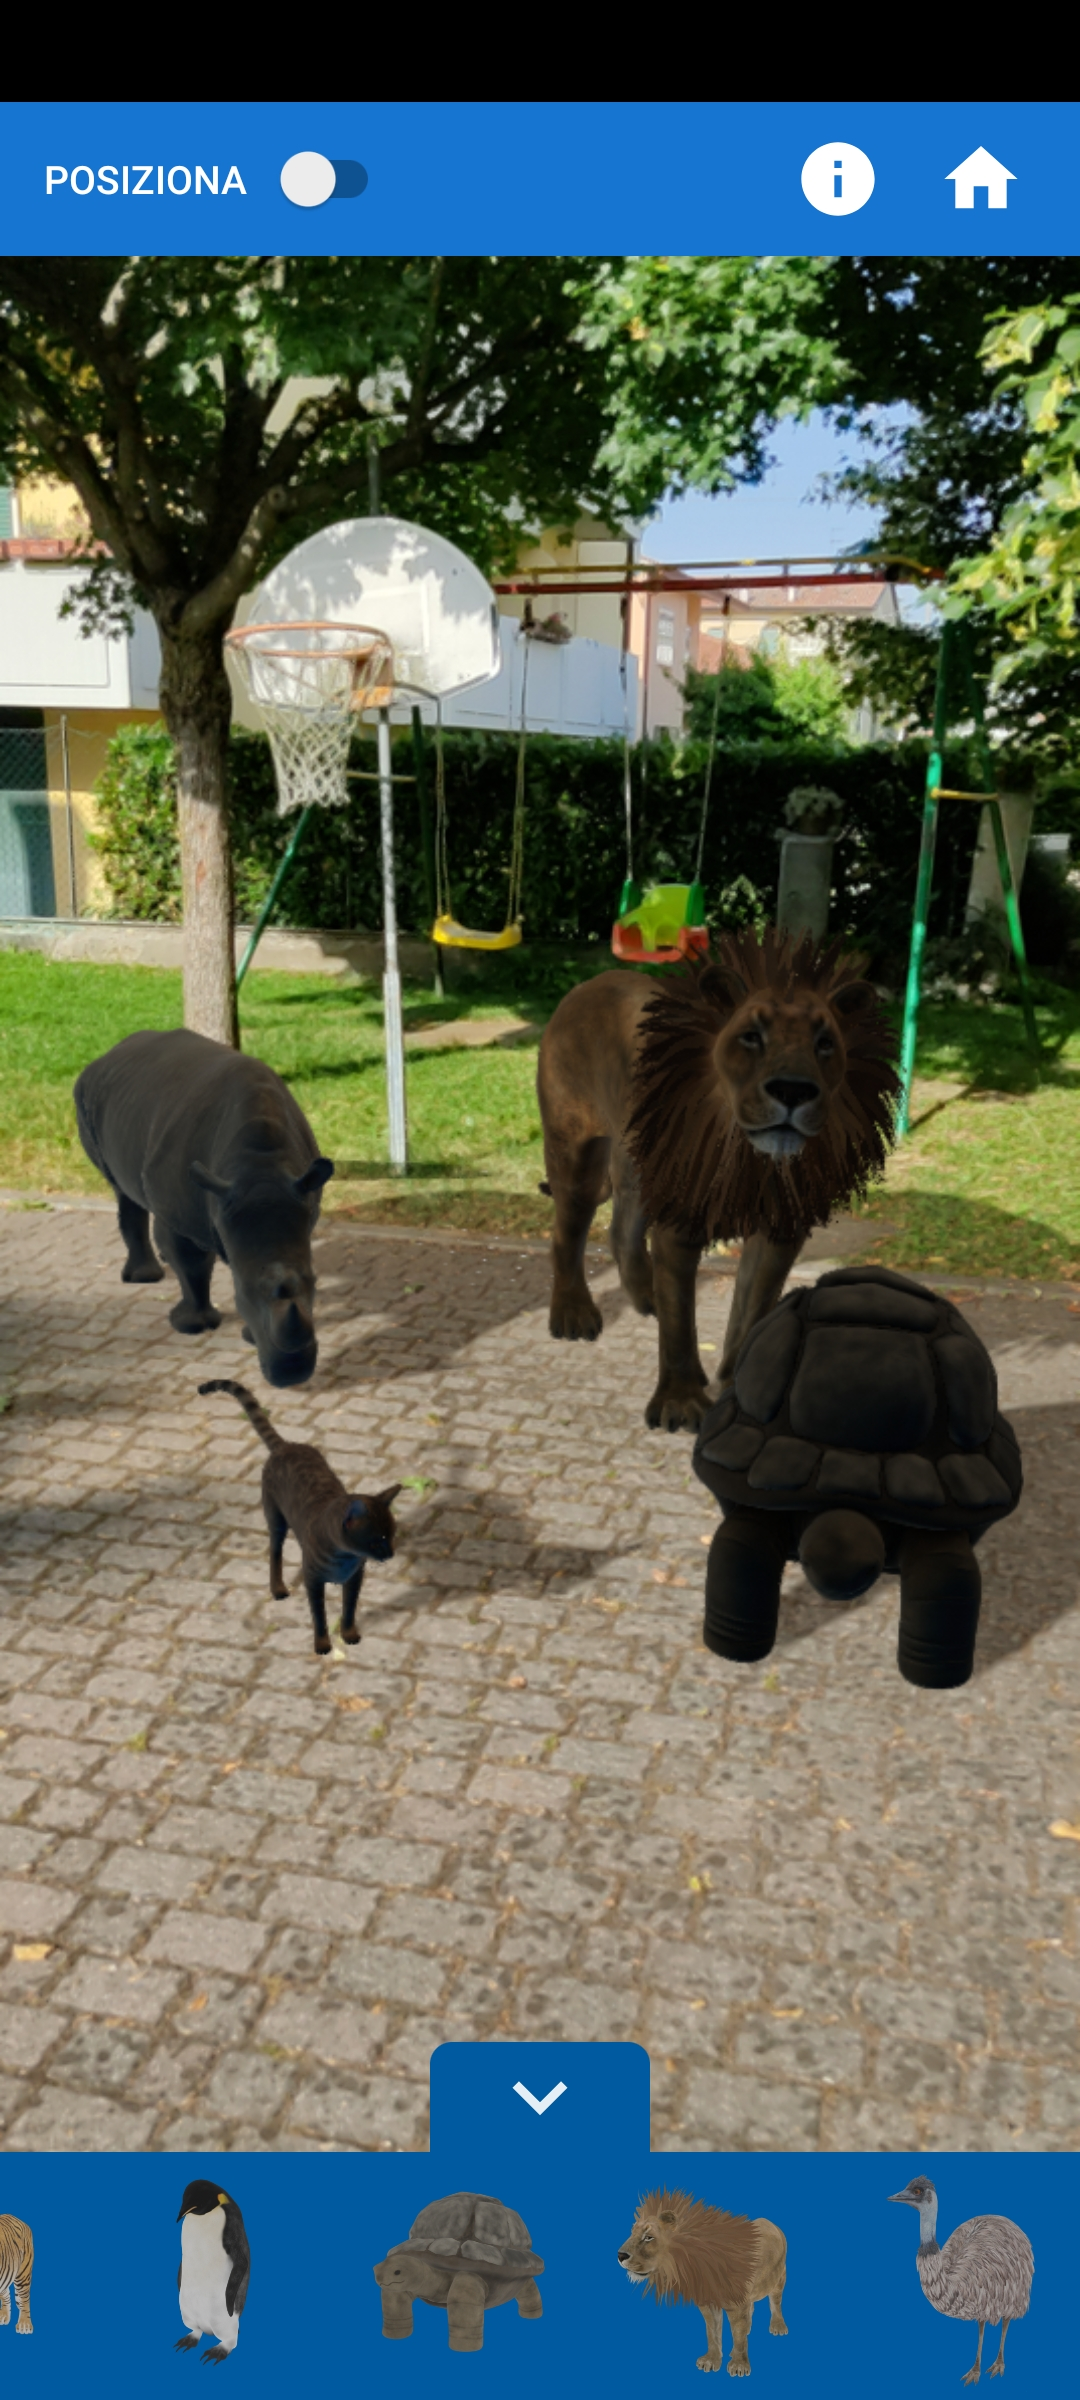
\includegraphics[width=0.3\textwidth]{./resources/images/UserInteraction/Animals2.jpg}} \qquad
			\caption{Esempio di molteplici hitTest su un piano in Plane Detection.}
			\label{fig:pet_img}
	\end{figure}
	
	\noindent
	Un potenziale test per stimare le performance dell'interazione con l'utente potrebbe consistere nel posizionare un numero notevole di oggetti virtuali nella scena ed esaminare se le performance diminuiscono con l'incremento del numero di oggetti. Si potrebbe scoprire se esiste una soglia di numero di oggetti per la quale l'applicazione si arresta. Si consiglia di eliminare anchor inutili per evitare che le performance diminuiscano notevolmente.

			
	
\end{document}